\begin{center}
\textsc{Gauss} an \textsc{Olbers}.\quad Zeven, 4.~Juli 1824.
\end{center}

\par\noindent\hspace*{\parindent}.\ .\ .\ .\ .\ .\quad Für weiteres Fortschreiten sind die Aussichten äußerst schlecht.
Nach meiner früheren Hoffnung Bremen zu umgehen, wird nicht tunlich sein, da
\par\smallskip\noindent\rule{.24\linewidth}{.4pt}\par\smallskip
{\footnotesize\noindent\hspace*{2.75em}[\textsuperscript{*}) Siehe die Briefe an \textsc{Olbers} vom 6.~Juli 1824, S.~320 Anmerkung, und vom 1.~März 1827, S.~378.]\par}
\par\smallskip\noindent{\footnotesize IX.}\hfill{\footnotesize47}\par
\clearpage
\noindent370\hfill{\small\textbf{BRIEFWECHSEL MIT OLBERS.}}\par\medskip
\noindent der Weierberg mit Brüttendorf nicht zu verbinden ist.
Aber auch \textls[120]{gar nichts} anderes Brauchbares lässt sich mit Brüttendorf im Nordwesten oder Norden verbinden.
\textsc{Müllers} Rekognoszierung von Bremervörde bis Osterholz hat durchaus \textls[120]{gar kein} Resultat gegeben.
Der einzige Punkt wäre bei Wentel, der aber an Bremen wohl nur einen Winkel von etwa \(12^{0}\), an Brüttendorf einen von \(46^{0}\), an Wentel von \(122^{0}\) p[raeterpro]pter geben würde, und wo ich auch noch gar nicht weiß, ob das Opfer, was ich durch ein so schlechtes Dreieck brächte
\par
\begin{center}
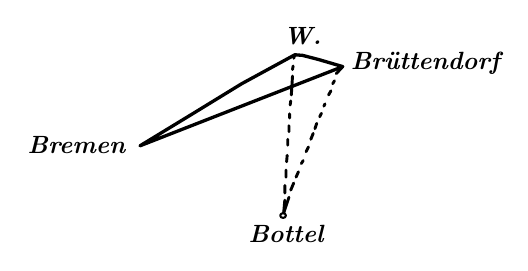
\begin{tikzpicture}[x=.0075cm,y=-.0075cm,line cap=round,line join=round]
\coordinate (Bremen) at (228,231);
\coordinate (Wentel) at (490,77);
\coordinate (Bruettendorf) at (571,97);
\coordinate (Bottel) at (470,349);
\draw[line width=1.2pt]
  (Bremen) -- (320,175) -- (400,126) -- (Wentel)
  -- (503,78) -- (530,85) -- (Bruettendorf) -- cycle;
\draw[line width=1.05pt]
  (Wentel) -- (488,83)
  (487,96) -- (486,102)
  (486,113) -- (484,145)
  (483,155) -- (482,162)
  (481,177) -- (481,184)
  (480,197) -- (480,207)
  (478,220) -- (478,230)
  (477,247) -- (476,258)
  (475,272) -- (475,284)
  (473,298) -- (473,311)
  (473,323) -- (471,345);
\draw[line width=1.05pt]
  (Bruettendorf) -- (560,109)
  (557,121) -- (554,126)
  (551,138) -- (547,145)
  (541,160) -- (539,164)
  (535,176) -- (532,182)
  (527,193) -- (524,202)
  (521,210) -- (517,220)
  (513,233) -- (509,241)
  (504,256) -- (501,261)
  (496,275) -- (492,284)
  (488,294) -- (483,306)
  (480,318) -- (471,345);
\draw[line width=.75pt,fill=white] (Bottel) ellipse [x radius=.36mm,y radius=.30mm];
\node[font=\small\bfseries\itshape,inner sep=0pt,anchor=east] at (204,229) {Bremen};
\node[font=\small\bfseries\itshape,inner sep=0pt,anchor=south] at (503,61) {W.};
\node[font=\small\bfseries\itshape,inner sep=0pt,anchor=west] at (584,92) {Brüttendorf};
\node[font=\small\bfseries\itshape,inner sep=0pt,anchor=north] at (475,365) {Bottel};
\end{tikzpicture}
\end{center}
\noindent (und welches etwas gebessert würde, wenn sich Wentel zugleich mit Bottel verbinden ließe), durch eine einigermaßen brauchbare Aussicht nach Nordwesten von Wentel aus kompensiert würde.
Am Ende werde ich also doch vielleicht den Steinberg noch hinzuzuziehen müssen, um mich südöstlich um Bremen herum zu drehen, oder Bremen nur wie eine vorgeschobene Zunge betrachten und die Verbindung mit \textsc{Krayenhoff} nördlich über Stade, oder südlich über Osnabrück suchen müssen.
Das erstere \textls[120]{allein} zu tun, ist wegen der unerhört schlechten Beschaffenheit der nordöstlichen \textsc{Krayenhoff}schen Dreiecke (worüber ich Ihnen früher einmal geschrieben) auch wohl bedenklich.
Sehr wünschte ich Ihre Ansicht darüber zu haben .\ .\ .\ .\ .\ .
